\subsection{Multi-agent adaptation}\label{sec:ma_adaptation}

\begin{figure}[h!]
    \centering
    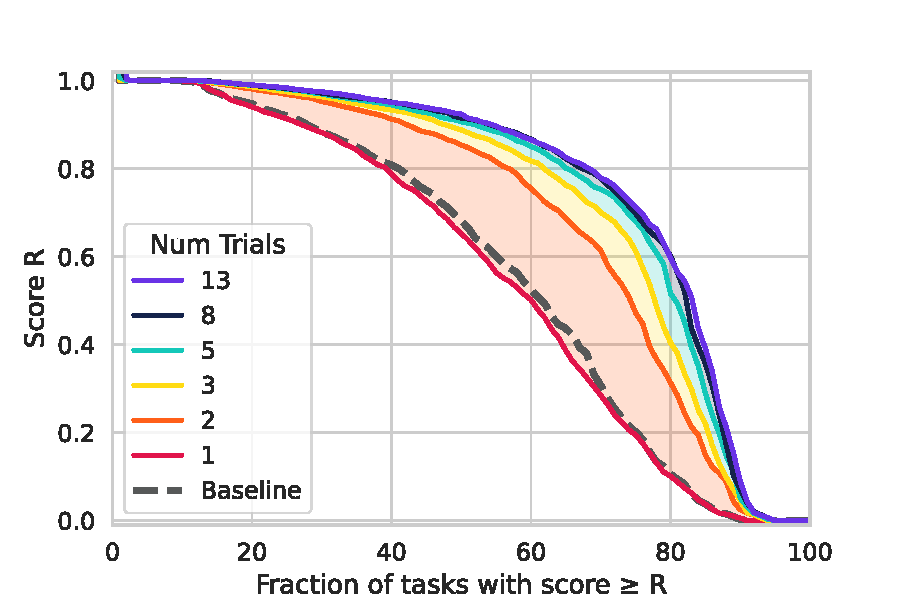
\includegraphics[width=0.6\linewidth]{figures/percentiles_vs_normalized_score_multi_agent.pdf}
    \caption{We report the distribution of normalised task scores over the multi-agent task test set when evaluated with various numbers of trials. All tasks are evaluated in cooperative self-play. On the $y$-axis is the total last-trial reward relative to that of an agent fine-tuned on the test tasks (approximating ``infinite trials'' performance). Curves moving further towards the top right corner indicate better performance. When given more trials, the agent achieves higher scores in the last trial, showing test-time adaptation across most of the task distribution (shaded regions). 
    }
    \label{fig:multi_agent_percentiles}
\end{figure}

\begin{figure}[h!]
    \centering
    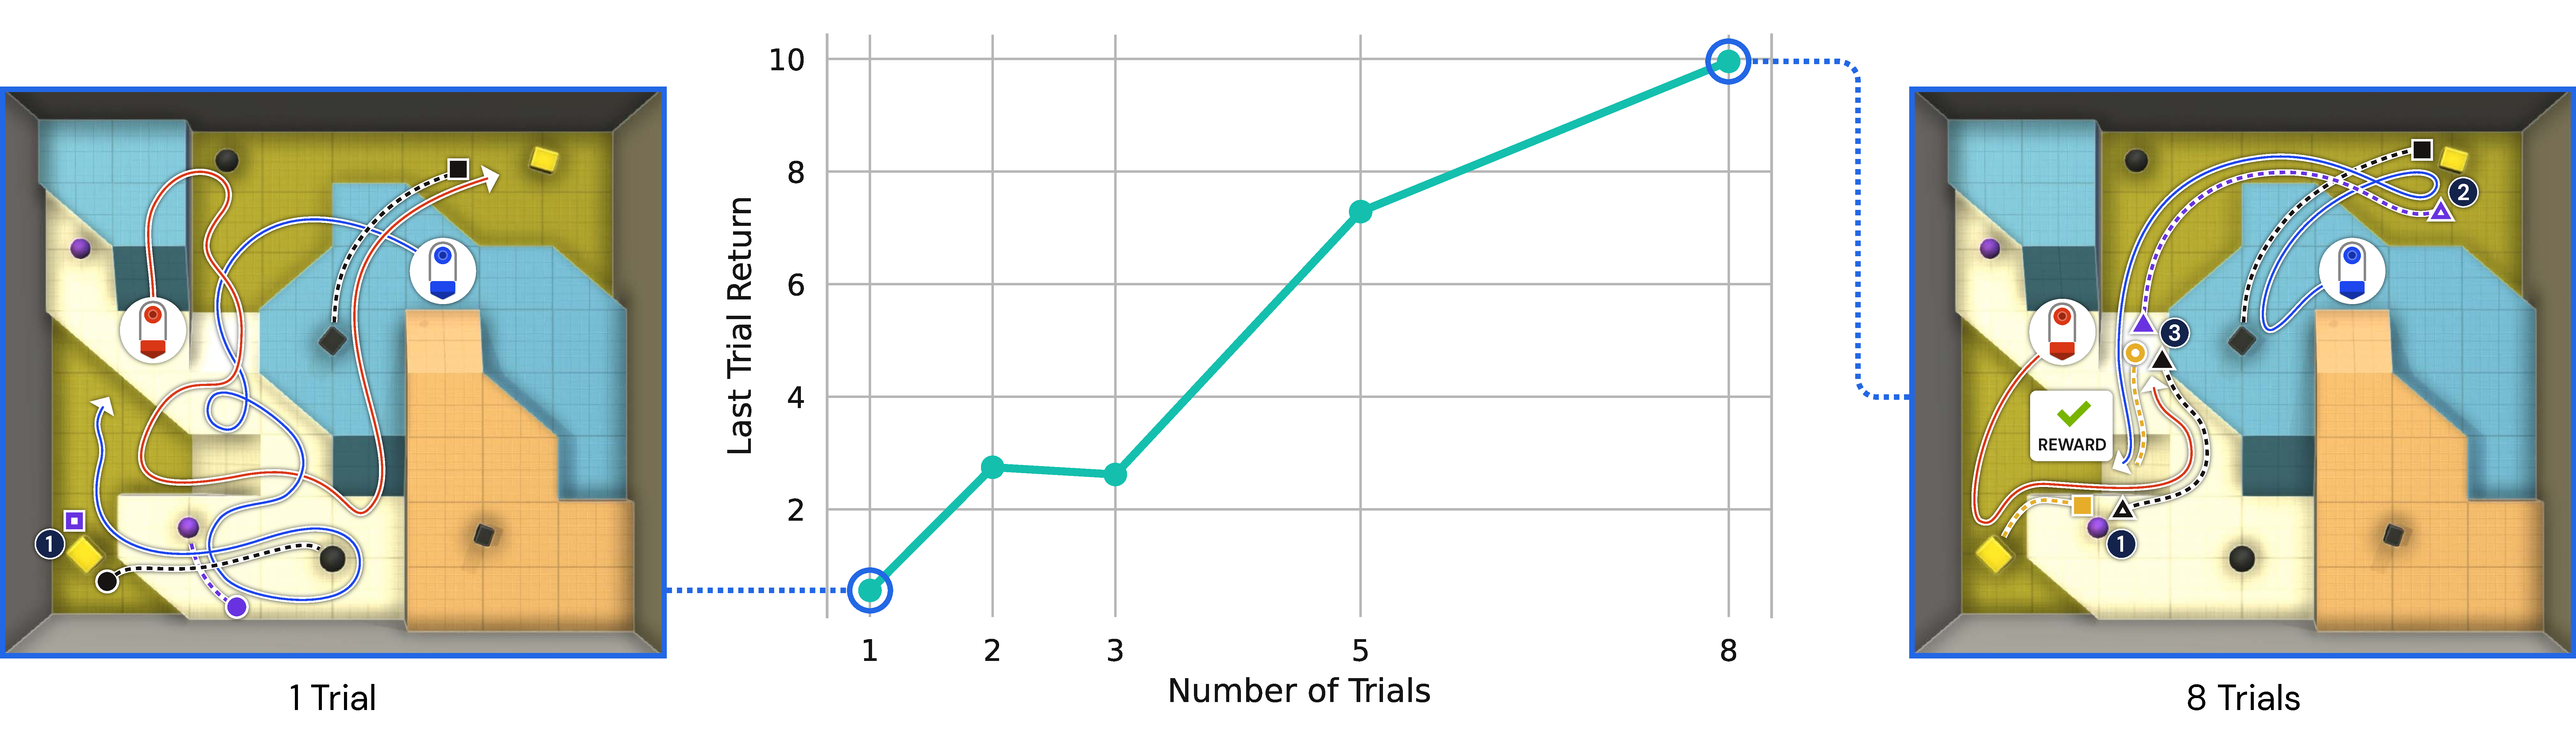
\includegraphics[width=1.0\linewidth]{figures/tasks/trajectories/trajectories_irreversible_production_for_two.pdf}
    \caption{Average performance and representative behaviour of AdA on the probe task \texttt{Irreversible Production for Two} when evaluated in self-play with various numbers of trials. AdA's performance increases when given more trials, showing test-time adaptation. The top-down view images show representative last-trial trajectories when given different numbers of total trials. A corresponding \href{https://youtu.be/hBc-7YMVo0U}{video} for the case $k = 8$ shows the behaviour across all trials within one episode.}
    \label{fig:multi_agent_probe_emergent_coop}
\end{figure}

Figure \ref{fig:multi_agent_percentiles} demonstrates adaptation across a wide range of percentiles on a test-task set of multi-agent tasks. Figure \ref{fig:multi_agent_probe_emergent_coop} demonstrates last-trial performance of AdA in one particular probe task. To generate these plots, AdA was trained as described in Section \ref{sec:results_human_scale_adaptation} (Multi-agent). 